\documentclass[12pt]{article}
\usepackage[utf8]{inputenc}
\usepackage{tipa}
\usepackage[margin=0.75in]{geometry}
\usepackage{enumitem}
\usepackage[center]{caption}
\usepackage{textcomp}
\usepackage{amsfonts}
\usepackage{amssymb}
\usepackage{amsmath}
\usepackage{amsthm}
\usepackage{mathrsfs}
\usepackage{float}
\usepackage{subcaption}
\usepackage{outlines}
\usepackage{graphicx}
\usepackage[dvipsnames]{xcolor}
\usepackage{color}
\usepackage{hyperref}
\hypersetup{
    colorlinks=false,
    linkcolor=SeaGreen,
    urlcolor=SeaGreen,
    linktoc=section}
\hypersetup{final=true}

\renewcommand{\qedsymbol}{Q.E.D.}
\renewcommand{\phi}{\varphi}
\DeclareMathOperator{\forces}{\Vdash}

\newtheorem{definition}{Definition}[section]
\newtheorem{theorem}{Theorem}[section]
% \newtheorem{kripkeModelDef}{Definition}

\begin{document}

\title{All Things Necessary and Possible: An Introduction to the Kripke Semantics of Modal Logic}
\author{M.~ R.~ Connor}
\date{13 September 2023}

\maketitle
\section{Key Definitions}

\begin{definition}
    A Kripke [\textipa{k\*rIpki}] frame $\mathfrak{F}$ is an ordered pair $(W, \mathcal{R})$, where $W$ is a non--empty set of possible worlds, and $\mathcal{R}$ is a relation
    between possible worlds called an \emph{accessibility relation}. This relation tells which worlds can access which other worlds.
\end{definition}

The possible worlds contain propositions, which are either sentence letters, or propositions built from the propositional logic connectives ($\sim$, $\wedge$, $\vee$, and $\rightarrow$) and 
the modal logic connectives $\square$ and $\lozenge$. We write $\mathcal{R}(\alpha, \beta)$ when the world $\alpha$ can access the world $\beta$. We read $\mathcal{R}(\alpha, \beta)$ as
``$\alpha$ can access $\beta$'' or as ``$\alpha$ sees $\beta$'' or as ``$\beta$ is accessible from $\alpha$''.

\begin{figure}[h]
    \centering
    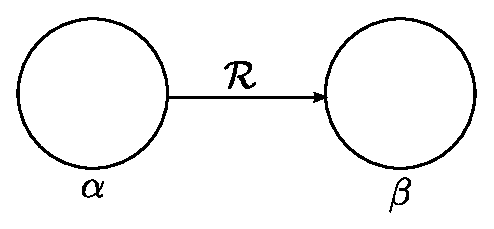
\includegraphics[width=2in]{Rab.eps}
    \caption{This type of diagram will be used throughout the notes, with the omission of the label of the arrow when it is clear that this refers to the accessibility relation. Here, we would
    read the relationship between the possible worlds as ``$\alpha$ sees $\beta$'', or as any of the other readings given above.}
    \label{Sample Kripke Frame}
\end{figure}

Figure \ref{Sample Kripke Frame} shows an example of how Kripke frames (as well as Kripke models) will be depicted in these notes: circles
will represent possible worlds and are labelled with letters from the beginning of the Greek alphabet, and arrows will represent the accessibility relation
and will not be labelled with the calligraphic $\mathcal{R}$ unless it is not clear that this represents the accessibility relation.

\begin{definition}
    A Kripke model $\mathfrak{M}$ is an ordered pair $(\mathfrak{F}, \forces)$, where $\mathfrak{F}$ is a Kripke frame and $\forces$ is 
    \emph{valutation operation} on propositions that assigns a truth value to the propositions in the Kripke frame. Classically, these truth values
    are \emph{true} and \emph{false}, but these are not the only possibilities that are seen in the literature.
\end{definition}    

Notice that Kripke models differ from Kripke frames in that they have this valuation operation. The way the valuation is expressed is $\alpha \forces
\phi$, and this is read as ``$\alpha$ satistifes $\phi$''. Other acceptable readings are ``$\alpha$ forces $\phi$'' and ``$\phi$ is true
in $\alpha$''. I like to think that the Kripke frame gives the Kripke model its body, and the valuation opeation gives it its soul.

\section{Extensional and Intensional Connectives}

The extensional connectives in modal logic are those that you know and love from propositional logic: the negation ($\sim$), the conjunction,
($\wedge$), the disjunction ($\vee$), and the material conditional ($\rightarrow$). These connectives are called \emph{extensional}. This means
that the truth value of the entire proposition can be determined from the truth value of its parts, down to the truth value of individual sentence
letters.

\begin{table}[h]
    \centering
    \begin{tabular}{| c | c | c |}
        \hline
        & \emph{When we say...} & \emph{...we mean} \\
        \hline
        $P$ & $\alpha \forces P$ & $P$ is true in world $\alpha$ \\
        \hline
        $\sim$ & $\alpha \forces \sim \! \phi$ & \textsc{Not}($\alpha \forces \phi$) \\
        \hline
        $\wedge$ & $\alpha \forces \phi \wedge \psi$ & $\alpha \forces \phi$ \textsc{And} $\alpha \forces \psi$ \\
        \hline
        $\vee$ & $\alpha \forces \phi \vee \psi$ & $\alpha \forces \phi$ \textsc{Or} $\alpha \forces \psi$ \\
        \hline
        $\rightarrow$ & $\alpha \forces \phi \rightarrow \psi$ & (\textsc{Not}($\alpha \forces \phi$)) \textsc{Or} ($\alpha \forces \psi$) \\
        \hline
    \end{tabular}
    \caption{This table shows how the syntax (structure) and semantics (meaning) of the extensional connectives behave. In the first row of the 
    table, $P$ could be any sentence letter.}
    \label{Extensional Table}
\end{table}

In Table \ref{Extensional Table}, we examine how the truth of a proposition built from extensional connectives in a Kripke model depends on the
truth of the components alone. For those who know the terminology, the connectives in the second column are in the object language,
and the connectives in the third column are in the metalanguage. For this reason, they are distinguished in notation.

\bigskip

The modal connectives, $\square$ and $\lozenge$, are not like this, however. They are \emph{intensional} connectives, meaning that we need more than
just the truth values of their components to determine the truth or falsity of the entire proposition. Their definitions in a Kripke model are given
in the table below, Table \ref{Intensional Table}.

\begin{table}[h]
    \centering
    \begin{tabular}{| c | c | c |}
        \hline
        & \emph{When we say...}& \emph{...we mean} \\
        \hline
        $\square$ & $\alpha \forces \square \phi$ & $\forall \beta \in W(\mathcal{R}(\alpha, \beta) \Rightarrow \beta \forces \phi)$ \\
        \hline
        $\lozenge$ & $\alpha \forces \lozenge \phi$ & $\exists \beta \in W(\mathcal{R}(\alpha, \beta)$ \textsc{And} $\beta \forces \phi)$ \\
        \hline
    \end{tabular}
    \caption{This table shows the relationship between the structure and meaning of the two modal connectives that we are interested in.}
    \label{Intensional Table}
\end{table}

The diagram in Figure \ref{Box Picture} shows what it looks like for a possible world in a Kripke model to force $\square \phi$. 
\begin{figure}[H]
    \centering
    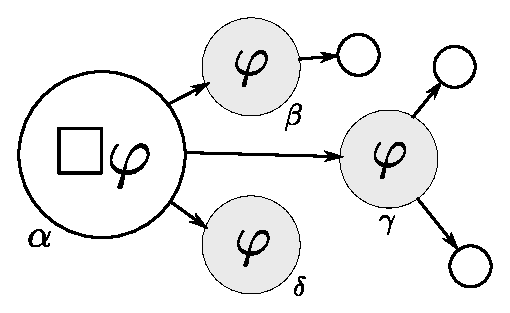
\includegraphics[width=2.5in]{box.eps}
    \caption{This figure shows how when a possible world (in this case, $\alpha$) forces $\square \phi$, \emph{each} accessible possible world 
    (in this case, $\beta, \gamma,$ and  $\delta$) must
    force $\phi$. Note that the possible worlds accessible from these need \emph{not} necessarily force $\phi$.}
    \label{Box Picture}
\end{figure}
Contrast this figure with the diagram in Figure \ref{Diamond Picture}, which shows what it looks like for a possible world to force $\lozenge \phi$.

\begin{figure}[h]
    \centering
    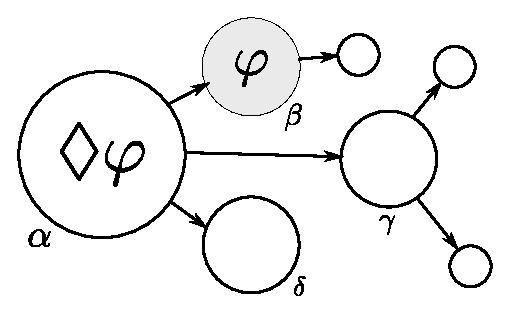
\includegraphics[width=2.5in]{diamond.eps}
    \caption{This figure shows how when a possible world (in this case, $\alpha$) forces $\lozenge \phi$, \emph{at least one} accessible
    possible world (in this case, $\beta$) must force $\phi$. Note that the possible world accessible from here need \emph{not}
    necessarily force $\phi$.}
    \label{Diamond Picture}
\end{figure}

\section{Interpretations of Modal Connectives}
Philosophers, logicians, mathematicians, and linguists are interested in modal logic for its ability to model a diverse
variety of systems that they like to reason about. For example, some philosophers like to think about ethics, and some linguists like to
think about how knowledge works and is updated as new information is introduced to an agent. These people use different interpretations of
$\square$ and $\lozenge$ to suit their needs. These are shown in the table below, along with several others which may be of interest.

\begin{table}[h]
    \centering
    \begin{tabular}{| c | c |}
        \hline
        $\lozenge \phi$ & $\square \phi$ \\
        \hline
        it is possible that $\phi$ is true & it is necessary that $\phi$ is true \\
        \hline
        $\phi$ is permissible & $\phi$ is obligatory \\
        \hline
        $\phi$ is consistent with an agent $A$'s knowledge & $\phi$ is known by an agent $A$ \\
        \hline
        $\phi$ is consistent in a system $\mathcal{S}$  & $\phi$ is provable in a system $\mathcal{S}$ \\
        \hline
    \end{tabular}
    \caption{This table shows the alethic, deontic, epistemic, and provability interpretations of the two modal connectives.}
    \label{Interpretations}
\end{table}

Table \ref{Interpretations} show some of the ways that logicians and non-logicians think about the modal connectives. Philosophers are mostly
interested in the first three interpretations. Linguists are mostly interested in the first and third. And mathematicians and logicians usually
want to know about the fourth interpretation. These interpretations inform the rationale for the modal axioms that we will discuss in the 
next section.

\section{Modal Axioms and the Kripke Semantics}

In order for the two modal connectives to model the scenarios that the logicians and non-logicians are interested in, they impose \emph{modal
axioms} on their Kripke models to do so. These are not axioms in the Euclidean or Peano senses, but in that we simply assume them as starting 
points for reasoning in our Kripke models. For example, a philosopher might want it to be the case that if something is obligatory, it is
obligatory that it is obligatory. So, the associated axiom they would be interested in would likely be the \textbf{4} axiom, named for 
System Four of C. I. Lewis. This axiom, stated in symbols is the following: $\square \phi \rightarrow \square \square \phi$. 

Compare this example with the previous: a mathematician interested in provability might want it to be the case that if something is provable, 
then it is true. (Clearly by the Incompleteness results, the converse is false.) They would perhaps wish to impose the \textbf{T} axiom on 
their Kripke models. This axiom, written symbolically, would be $\square \phi \rightarrow \phi$. 

A mysterious correspondence appears when we look at what happens when we endow our Kripke models with axioms and look at the accessibility
relation of the associated Kripke frame. For example, if our Kripke model is endowed with the \textbf{T} axiom, the accessibility 
relation on the associated Kripke frame becomes reflexive without us having to do anything else. The converse is also true. We will prove the 
first statement by picture. The proof of the converse is given in the bonus section. 

\begin{theorem}
    The \textbf{T} axiom is true in a Kripke model only if the associated Kripke frame has a reflexive accessibility relation.
\end{theorem}

\begin{proof}
    We will proceed by contraposition. Let $\mathfrak{M}$ be a Kripke model. Assume that the \textbf{T} axiom is false at some 
    world in our $\mathfrak{M}$. Then it is the case that $\sim \! \!(\square \phi \rightarrow \phi)$ is true in this world. By the negation of
    the condtional, we find that this is equivalent to stating that $\sim \! \phi \wedge \square \phi$ is true (Subfigure \ref{Proof Step 1}). We can separate the conjuncts
    to allow us to more easily work with them. (Subfigure \ref{Proof Step 2}) By the definition of $\square$ given in Table \ref{Intensional Table}, we know that $\phi$
    must be satisfied by all possible worlds accessible from the one that satisfies $\square \phi$. (Subfigure \ref{Proof Step 3})
    
    \begin{figure}[h]
        \centering
        \begin{subfigure}{0.27\textwidth}
            \centering
            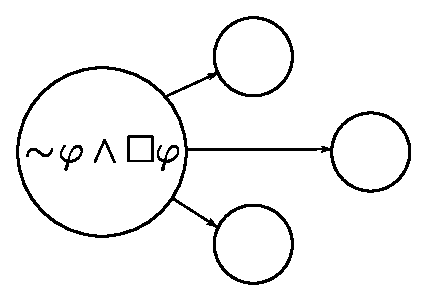
\includegraphics[width=\textwidth]{proof1.eps}
            \caption{This shows our \\ assumption for contraposition.}
            \label{Proof Step 1}
        \end{subfigure}
        \begin{subfigure}{0.27\textwidth}
            \centering
            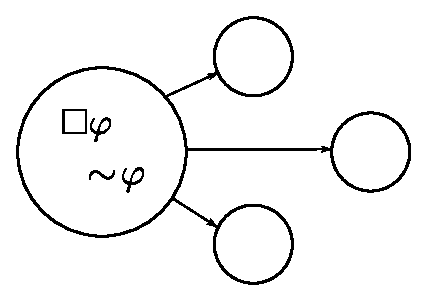
\includegraphics[width=\textwidth]{proof2.eps}
            \caption{Here we have separated \\ the two conjuncts.}
            \label{Proof Step 2}
        \end{subfigure}
        \begin{subfigure}{0.27\textwidth}
            \centering
            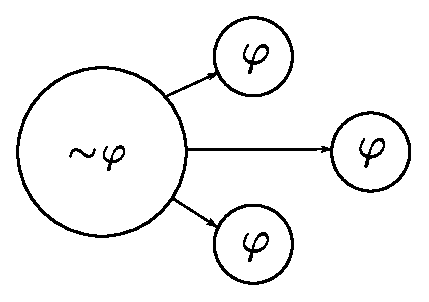
\includegraphics[width=\textwidth]{proof3.eps}
            \caption{We have used the definition of $\square \phi$.}
            \label{Proof Step 3}
        \end{subfigure}
        \caption{These are the first three major steps in our proof}
        \label{Proof Step 1-3}
    \end{figure}
    
    But it can not be satisfied by the one
    that satisfies $\square \phi$ itself, for that world contains $\sim \! \phi$, which would cause a contradiction. 
    \begin{figure}[h]
        \centering
        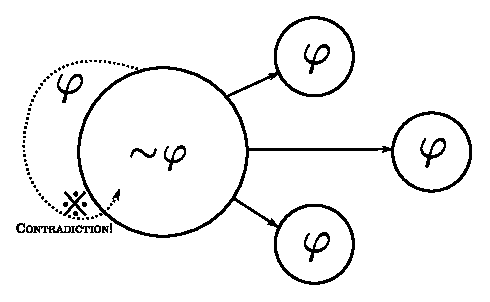
\includegraphics[width=0.4\textwidth]{proof5.eps}
        \caption{This shows us that the world which forces $\square \phi$ cannot also force $\phi$ without contradiction.}
        \label{Contradiction}
    \end{figure}

    Thus, this world is not accessible from itself. So the accessibility relation in the underlying Kripke frame cannot be reflexive. (Figure \ref{Contradiction})
\end{proof}

This is not the only correspondence of its kind! These are called the Kripke Semantics of modal logic, and they give both structure and meaning to
Kripke frames and models. They give connection between Kripke frames, which are fundamentally syntactic, and Kripke frames, which have a more
semantic basis for their existence. Other examples from the Kripke Semantics include that the \textbf{4} axiom gives the associated Kripke frame 
a transitive accessibility relation. 

Multiple axioms can be given to the Kripke model at once, forming a modal system. One of the most famous of these is called \textbf{S5}, and it
is favored by philosophers and mathematicians for its accessibility relation which is an equivalence relation. This modal system has been
equipped with the axioms \textbf{K}, \textbf{T}, \textbf{B}, and \textbf{4}. (See the bonus section for the statements of these in symbols.) Lest the reader
believe that the Kripke Semantics must always produce an accessibility relation described in first--order logic, here is an example of an axiom
with the following properties, the second of which is non--first--order: the \textbf{L} axiom, which is both transitive and converse--well--founded.
(Converse--well--foundedness means that $\mathcal{R}^{-1}$ is well--founded.) The \textbf{L} axiom is the following statement:
$$\square (\square \phi \rightarrow \phi) \rightarrow \square \phi.$$ This axiom is the one that can lead to a proof of the First Incompleteness
result.

\section{What to Explore Next}
Here is a brief list of things that the reader may wish to explore next, if interested in learning more about modal logic. 

\begin{itemize}[noitemsep]
    \item Bisimulations are a sort of homomorphism between Kripke models. They allow us to make statements that are true for Kripke models 
    with a certain structure. There are ways to think about them in terms that are useful to graph theorists, computer programmers, philosophers, and
    logicians.
    \begin{itemize}[noitemsep]
        \item P-morphisms (short for \emph{pseudo-epimorphisms}, but no one calls them that) are a special variety of bisimulation.
        \item Van Benthem's [\textipa{fan bEnt\textsuperscript{h}@m}] Theorem states that modal logic is precisely the fragment of
        first--order logic invariant under bisimulation. To find out what this means, see the resources in the next section.
    \end{itemize}
    \item The Sahlqvist-van Benthem Algorithm gives a constructive and deterministic way to go to the first--order formula promised by van Benthem's
    from a given modal formula.
    \item In the words of van Benthem, ``There is a whole garden of modal systems to explore. However, only some are interesting. 
    How can you tell? If you lack soundness and completness in your system, you have nothing.'' Thus, it would seem that proving soundness and completness
    for modal systems like \textbf{S5} is important, and leaves many things to be found still in modal logic.
\end{itemize}

\section{My Book Recommendations for the Interested Reader}
Here are the books which guided and still guide me through the landscape of modal logic. There are many others out there, but these three
were the most influential on my journey. These opinions are solely my own and do not reflect the objective qualities of the books. In no particular order:

\begin{itemize}[noitemsep]
    \item \emph{Modal Logic for Open Minds}, J. van Benthem.
    \begin{itemize}[noitemsep]
        \item Fun, lighthearted introduction to the subject.
        \item Explores many of the different applications of modal logic in some depth, though not as much as the book below.
        \item Has good exercises, but there aren't a lot per chapter.
    \end{itemize}
    \item \emph{Modal Logic}, P. Blackburn, M. de Rijke, Y. Venema (all academic sons of van Benthem).
    \begin{itemize}[noitemsep]
        \item A more serious and rigorous dive into the subject, appropriate after some study of logic.
        \item The standard textbook for modal logic at the University of Amsterdam's Introduction to Modal Logic course.
        \item Moves a bit fast.
    \end{itemize}
    \item \emph{Boxes and Diamonds}, many contributors through the Open Logic project.
    \begin{itemize}[noitemsep]
        \item Can be downloaded in full in either pdf or \LaTeX \: format and tweaked to your notation and style preferences.
        \item Lots of diagrams.
        \item Color version may be taxing to print.
    \end{itemize}
\end{itemize}

\section{Bonus!}
Here are some things that didn't seem to belong in the main part of the talk/notes. They have been farmed out to this bonus section for the 
enjoyment of the curious/pedantic reader.

\subsection{Proof of the other direction of the biconditional from Section 4}
\begin{theorem}
    The Kripke frame associated with a Kripke model has a reflexive accessibility relation only if the \textbf{T} axiom is imposed on the model.
\end{theorem}

\begin{proof}
    Let us work in a Kripke frame $\mathfrak{F}$. Suppose for contraposition that its accessibility relation is not reflexive. Then it must be
    the case that there is some world $\alpha$ which does not see itself, that is, there exists some $\alpha$ such that $\sim \! \! R(\alpha, \alpha)$.
    Let us define a Kripke model $\mathfrak{M}$ on $\mathfrak{F}$ and let $\phi$ be a proposition. Let our valuation operation in $\mathfrak{M}$
    be such that $\phi$ is true in every world in $\mathfrak{F}$ except the irreflexive one, $\alpha$. Thus we know that in all worlds that are
    accessible from $\alpha$, $\phi$ is true. So we have that $\alpha \forces \square \phi$ and $\alpha \forces \sim \! \! \phi$. So by the
    negation of a conditional used in reverse, we know that this is equivalent to $\alpha \forces \sim \! \! (\square \phi \rightarrow \phi)$. 
    This is precisely the negated \textbf{T} axiom. This has shown us that if a world is made to be incaccesible from itself, then the \textbf{T} axiom
    cannot be true for the entire Kripke model. Thus, by the contrapositive, we have the theorem.
\end{proof}

\subsection{More Kripke Semantics correspondences}
The table below shows more Kripke Semantics correspondences than would fit or be relevant to the above sections.

\bigskip
\centering
\begin{tabular}{| c | c | c |}
    \hline
    Name & Axiom & Kripke Semantics \\
    \hline
    \textbf{K} & $\square (\phi \rightarrow \psi ) \rightarrow (\square \phi \rightarrow \square \psi)$ & Allows for the use of \emph{modus ponens} \\
    \hline
    \textbf{B} & $\phi \rightarrow \square \lozenge \phi$ & symmetry of $\mathcal{R}$ \\
    \hline
    \textbf{D} & $\square \phi \rightarrow \lozenge \phi$ & seriality of $\mathcal{R}$ \\
    \hline
\end{tabular}

\end{document}